\subsubsection{SOLLVE} \label{subsubsect:sollve}


\paragraph{Overview} 

OpenMP is a   directive-based API for shared-memory and accelerator systems. It
is supported by a stable community of vendors, research labs, and academics who
participate in the efforts of the  OpenMP Architecture Review Board; it   is
also the most used API for intra-node programming in ECP applications.
Implementations are available in all DOE LCFs, and a variety of programming
tools are available to support OpenMP application development. The mission of
the SOLLVE project is to further enhance the OpenMP specification and
implementations to meet the performance and productivity goals of ECP
applications. We directly interact with DOE end-users in order to understand
their application software requirements. We will develop OpenMP solutions for
ECP needs; propose features for standardization; produce prototype
implementations of new features to support their rapid adoption; develop and
deliver a verification and validation (V\&V) suite to assess implementations and
enable evaluations by DOE  facilities, and deliver a high-quality,  robust ECP
OpenMP implementation in the LLVM compiler framework. Attaining high levels of
single-node performance and meeting performance portability needs will only be
possible via enhancements to OpenMP in such areas as data motion and placement
in complex memory  hierarchies, efficiency in the context of C++,  and features
that allow the creation of performance portable code. SOLLVE plays a critical
role in identifying, implementing, promoting, and deploying key functionality
that will enable ECP application developers to reach their goals using OpenMP.
We will demonstrate the high impact of new features via their use in selected
ECP applications.

\paragraph{Key  Challenges}
%\textit{Describe what is hard to do, why it is challenging.}
The SOLLVE project addresses a number of key challenges faced by DOE facilities,
application groups and scientists. The first of these is the gap between
existing OpenMP functionality and user requirements. This problem is largely
exacerbated by ever increasing complexity and heterogeneity of computing
systems.
The second challenge is to suitably evolve the OpenMP specification to satisfy
the identified requirements. This process involves coordinating with vendors
and other members of OpenMP's language committee  to reach consensus on the scope of the API, syntax and semantics of new features.
The third challenge addressed by the SOLLVE project is performance portability.
Current hardware and software trends 
\cite{exascale-roadmap.ijhpca.2011}
 have shown that
pre-Exascale and Exascale systems will be extremely heterogeneous, and may 
consist of  diverse architectures such as
CPUs, GPUs, FPGAs, among others. Programmatically, this means that 
memory hierarchies will be even deeper, and multiple levels and types
of parallelism will have to be exposed, extracted and mapped onto these systems 
to achieve suitable performance levels. 
This naturally places heavy emphasis on application readiness, where APIs such as 
OpenMP will need to address 
performance portability to serve the critical role
of abstracting hardware and software complexities.
Finally, the last challenge is to fully assess the quality of delivered
OpenMP implementations, their compliance with the specification and potential
divergence that, if unidentified, could can lead to undesired program behavior.
% and, ultimately, errors
%that can consume significant amount of resources to repair.


\paragraph{Solution Strategy}
The challenges discussed here are addressed by 5 major thrust areas, which
we describe below as part of the SOLLVE process:
%\textit{Describe your basic strategy for addressing the challenges.}

\begin{enumerate}
\item {\bf Application requirements}
The first step of the SOLLVE process consists in collecting user requirements
from relevant and representative ECP applications (e.g. QMCPACK or Lattice QCD).
Collected requirements are then converted to use-cases which are then handed
to the OpenMP Standard Committee.
\item {\bf OpenMP specification evolution}
This thrust area is responsible of translating use-cases to new OpenMP
features to be introduced into the standard. In this phase, the semantics
of the new capabilities are defined and formalized, followed by early
prototypes in one or more OpenMP implementations (either vendor or open
source solutions). Broadly, the bulk of new features fall into the areas
of accelerator, affinity, tasking or memory management.
\item {\bf Lightweight OpenMP runtime}
SOLLVE is committed to deliver an open source, lightweight and scalable
OpenMP implementation (the BOLT runtime) that will fulfill ECP needs.
This deliverable serves two key objectives: i) early access to a stable 
implementation; and ii) risk mitigation.
\item {\bf LLVM }
This compiler infrastructure is ideal for 
delivering high-quality and deployable OpenMP implementations.
Our effort enhances the LLVM framework by introducing compiler transformations
that leverage both prototyped OpenMP features and those introduced
in OpenMP 4.5. User adoption of new OpenMP capabilities could vary from
months to years. Thus, delivering compiler technology that automatically transforms
user's code targeting the new OpenMP functionality (e.g. target offloading with
data mappers), represents high return value for ECP in terms of time and
resources. 
\item {\bf Validation and verification (V\&V)} This thrust focuses on
designing and implementing a benchmark suite that allows to assess the coverage
and standard compliance of several OpenMP implementations (LLVM, BOLT, IBM XL,
NVIDIA, etc). In addition, a ticket system for bug reporting and inquiries has
also been deployed to facilitate interaction with end users.
\end{enumerate}

\paragraph{Recent Progress}
Figure \ref{fig:sollve-update} shows the latest progress on the 5 core SOLLVE
thrust areas. We note that the {\bf training and outreach} activity is a
cross-cutting effort which includes resources from the SOLLVE project and
external partners, namely collaborators from Lawrence Berkeley National
Laboratory, Oak Ridge, University of Delaware and other academic institutions.
In addition to the above updates, a number of articles have also been published
as part of the SOLLVE effort \cite{openmp-tr6,zinenko.cc.2018,osti_1429981,DBLP:conf/sc/MishraLKFC17}.

\begin{figure}[t]
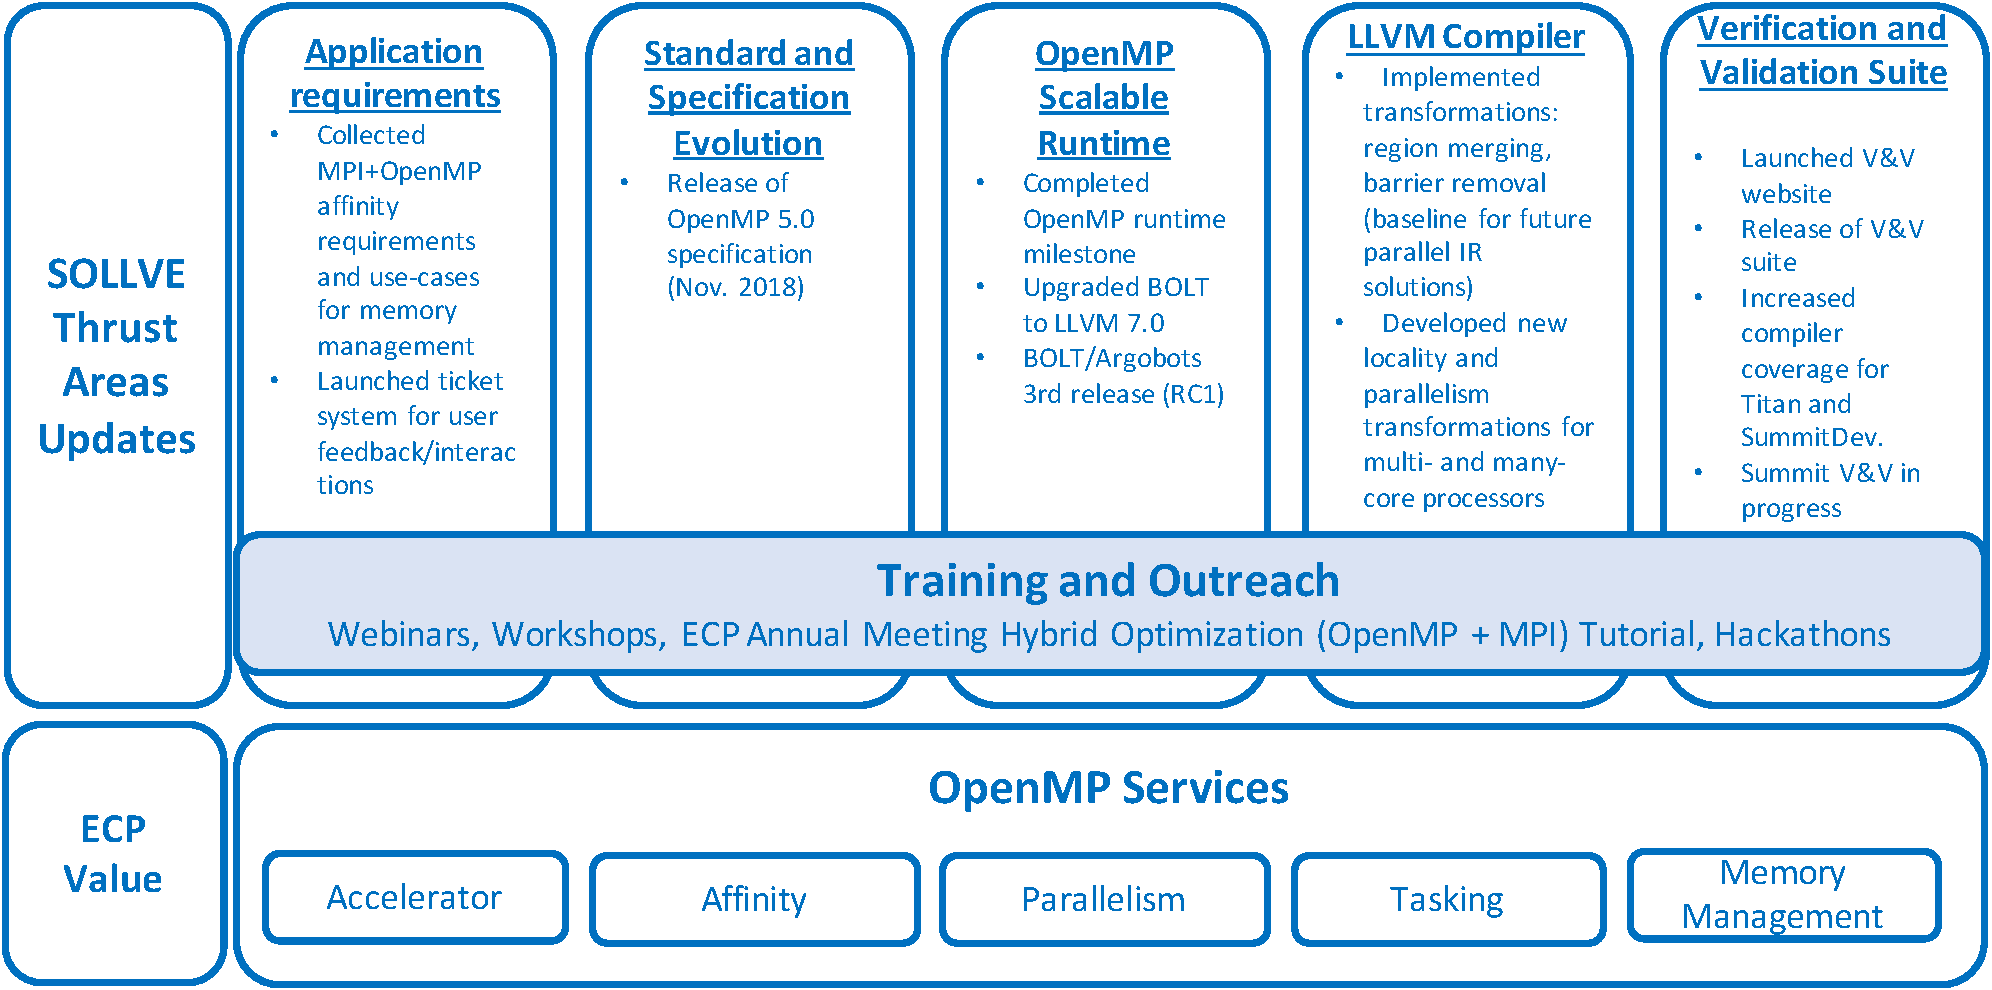
\includegraphics[width=0.98\linewidth,height=8cm]{projects/2.3.1-PMR/2.3.1.13-SOLLVE/SOLLVE-progress}
\caption{\label{fig:sollve-update}SOLLVE thrust area updates}
\end{figure}

\paragraph{Next Steps}
As next steps planned for SOLLVE we have
\begin{itemize}
\item Applications: gather more requirements for memory management API and concurrent parallel construct; prepare and coordinate OpenMP webinar focusing on memory management, deep copy and tasking.
\item OpenMP standard: Next face-to-face meeting in May; ratify and vote latest memory management features, mappers and parallelism descriptors
\item OpenMP runtime: design and implement high-level interface for passing scheduling/blocking hints
\item LLVM compiler: develop new optimizations leveraging prototype parallel-IR; refine Clang based implementation of data layout transformations; evaluate new compiler transformations on Intel KNL and ARM architectures
\item V\&V suite: identify performance critical kernels from selected applications; prepare release for SC18; coordinate suite deployment with CORAL systems.
\end{itemize}

